\documentclass[12pt]{book}
\usepackage{a4wide}
\usepackage{graphicx}
\usepackage{amssymb}
\usepackage{epstopdf}
\usepackage[hidelinks]{hyperref}
\usepackage{listings}
\usepackage{cite}
\usepackage{xcolor}
\usepackage{soul}
\DeclareGraphicsRule{.tif}{png}{.png}{`convert #1 `dirname #1`/`basename #1 .tif`.png}

\lstdefinestyle{BashInputStyle}{
  language=bash,
  basicstyle=\small\ttfamily,
  numbers=none,
  numberstyle=\tiny,
  numbersep=3pt,
  frame=none,%tb,
  columns=fullflexible,
  backgroundcolor=\color{yellow!20},
  linewidth=\linewidth,
  xleftmargin=0.0\linewidth,
  showstringspaces=false
}
\lstdefinestyle{mystyle}{
    backgroundcolor=\color{yellow!20},   % Background color
    basicstyle=\ttfamily\small,         % Font and size (Consolas)
    breaklines=true,                    % Wrap long lines
    captionpos=b,                       % Caption position (bottom)
    frame=none,                       % Frame around code
    numbers=none,                       % Line numbers on the left
    numberstyle=\tiny,                  % Style for line numbers
    showstringspaces=false              % Don't show spaces in strings
}
\lstdefinestyle{inlinecode}{
    backgroundcolor=\color{yellow!20},  % Background color
    basicstyle=\ttfamily,              % Font (Consolas)
    showstringspaces=false             % Don't show spaces in strings
}

% Shortcut for inline commands
\newcommand{\ilc}[1]{\colorbox{yellow!20}{\texttt{#1}}}

% Shortcut for inline keywords
\newcommand{\ilk}[1]{{\textbf{\textbf{#1}}}}

% Shortcut for inline options
\newcommand{\ilo}[1]{{\color{blue}\texttt{#1}\color{black}}}

% Define code blocks
%    \begin{lstlisting}[style=mystyle]  % Use your preferred style
%    \end{lstlisting}

%\textwidth = 6.5 in
%\textheight = 9 in
%\oddsidemargin = 0.0 in
%\evensidemargin = 0.0 in
%\topmargin = 0.0 in
%\headheight = 0.0 in
%\headsep = 0.0 in
%\parskip = 0.2in
%\parindent = 0.0in
%\bibliographystyle{unsrt}
\bibliographystyle{tlcpub2}

\newtheorem{theorem}{Theorem}
\newtheorem{corollary}[theorem]{Corollary}
\newtheorem{definition}{Definition}

\title{\textsc{NISE Manual\\ Version 3.4}}
\author{Thomas la Cour Jansen\\ University of Groningen}
%\date{\today\\ \includegraphics{2ds.pdf}}
\date{\today\\ \includegraphics{cover.png}}
\begin{document}
\maketitle

\thispagestyle{empty}
\rule{0mm}{0mm}
%\vfill
\noindent
\thispagestyle{empty}
Front cover: 
%\\[4ex]
%Thomas la Cour Jansen,\\[2ex]
\copyright \/ T.l.C. Jansen, 2017
\setcounter{page}{1}
\thispagestyle{empty}
\clearpage

\addcontentsline{toc}{chapter}{Contents}
\setcounter{page}{1}
\include{tableofcontents}
%\addtocontents{toc}{\protect\thispagestyle{empty}}
%\tableofcontents

\chapter{Introduction}
The main developer of the NISE3 code is Thomas la Cour Jansen. Please, cite the appropriate
references 
\cite{Jansen.2006.JPCB.110.22910,Jansen.2009.ACR.42.1405,Jansen.2010.JCP.132.224503,Liang.2012.JCTC.8.1706,Liang.2013.JPCL.4.448}
when publishing work using this code. The code allows the calculation of the linear absorption,linear dichroism, sum-frequency generation, two-dimensional spectra (IR,UVvis, and SFG), population transfer, exciton diffusion and integrated anisotropy using the full nonadiabatic semi-classical numerical integration of the Schr\"{o}dinger equation approach
\cite{Jansen.2009.ACR.42.1405} and the sparse matrix optimization approach \cite{Liang.2012.JCTC.8.1706}. The code allows treating spectra of diverse systems involving
intra- and intermolecular energy transfer\cite{Jansen.2006.JPCB.110.22910,Cringus.2007.JCP.127.084507,Jansen.2008.BJ.94.1818,Dijkstra.2010.JPCA.114.7315,Jansen.2010.JCP.132.224503}, non-Gaussian dynamics \cite{Jansen.2009.JPCA.113.6260,Roy.2011.JPCB.115.5431}, surfaces \cite{Liang.2013.JPCL.4.448}, and chemical exchange \cite{Jansen.2007.JCP.127.234502}. This manual is not intended as an introduction to two-dimensional
spectroscopy. The user is directed to the references including recent reviews \cite{Hamm.1998.JPCB.102.6123,Hochstrasser.2001.CP.266.273,Cho.2008.CR.108.1331,Mukamel.2000.ARPC.51.691,Jansen.2009.ACR.42.1405} and books
for more information \cite{Cho.2009.B01,Mukamel.1995.B01,Hamm.2011.B01}.

The code is made available as open source on github.com as link {\tt GHlacour/NISE\_2017}. The version available is intended to be friendly for developers to contribute improvements. Changes in the code are at own risk and should be reported clearly in publications. Developers wanting to contribute to the official version of the code are suggested to contact the main developer in advance to ensure that the contribution is not conflicting with that of other developers. More information for developers is given in Chapter \ref{chap:developers}. Feedback on the program and the manual are welcome via e-mail: t.l.c.jansen@rug.nl. 

Current developers include: Thomas la Cour Jansen (main developer), Floris Westerman (cmake and MPI implementation), and members of the Computational Spectroscopy group at the University of Groningen.

%The code use wavenumbers (cm$^{-1}$) for frequencies and times are femtoseconds (fs). The transition dipoles and transition polarizabilities may be given in any desired units in most cases, but Debye is recommended for transition dipoles and required for the coupling on the fly methods. Distances in that case should be given in Ångstrøm.

The code use wavenumbers (cm$^{-1}$) for frequencies and times are in femtoseconds (fs).  The transition dipoles should preferably be given in Debye and transition polarizabilities in \AA$^{3}$.  For using the on-the-fly coupling calculations the transition dipoles should be provided in Debye and positions should be provided in \AA ngstr\"{o}m. Users are discouraged from trying to use other units at this may lead to numerical instabilities or unit conversion errors. The final results will scale accordingly.

In this manual keywords used in the NISE input files are highlighted as \ilk{Keyword}. Variables defined with these keywords are highlighted as \ilo{variable}. Code to be typed in the linux command line or to be used in a script is highlighted as \ilc{code}.

\chapter{Installation and options}
A demonstration for installing NISE can be found on YouTube: \url{https://www.youtube.com/watch?v=npvV9UOFmDg&t=7s}.
NISE has a number of dependencies:
\begin{itemize}
\item FFTW3 library, possibly with OpenMP/MPI support. See \url{http://www.fftw.org/}.
\item LAPACK library, often preinstalled. See \url{http://www.netlib.org/lapack/}.
\item CMake v3.10 or higher
\item MPI v3 implementation, such as OpenMPI, MPICH (Unix) or MS-MPI (Windows)
\item Modern C compiler, implementing a recent OpenMP version
\item LaTeX + BibTex distribution if you want to build the documentation. Not required
\item DISLIN, python, MATLAB, or gnuplot, for plotting the results using the included scripts
\end{itemize}
As some FFTW3 installations do not come with the correct CMake compatibility, it might be useful to use \href{https://github.com/microsoft/vcpkg}{vcpkg} as package manager for C++ libraries. This package manager is cross-platform compatible.

\section{Building}
In order to build and compile the NISE software, it is recommended to use the CMake build system. This will try to automatically link the libraries and pick the correct compiler settings.
\begin{enumerate}
\item Extract the source code files.
\item Create a \texttt{build} directory in the main folder using \ilc{mkdir build}.
\item Run \ilc{cmake ..} inside this new \ilc{build} directory.
\item If \ilc{cmake} was successful, run \ilc{make} in the same directory to start compilation.
\item All executables should be available in a new \ilc{bin} directory in the main folder.
\end{enumerate}

\noindent
Additional steps to install on MacOS and Windows can be found in section 2.2.\\

There are several options you can provide to the \ilc{cmake} command in order to customize your build:
\begin{itemize}
\item \ilc{-DCMAKE\_BUILD\_TYPE}: By default, this is set to \ilc{ RelWithDebInfo}. Other options include \ilc{Debug}, \ilc{Release} and \ilc{MinSizeRel}. Refer to the CMake documentation for more information
\item \ilc{-DGENERATE\_DOCS}: When not set, CMake will attempt to compile this documentation only when building a Release build. You can override this by setting this variable to \ilc{true} or \ilc{false}.
\item \ilc{-DACCURATE\_MATHS}: When set, CMake will compile the code to use accurate mathematics implementations (as is default when using a C compiler). When not set, the compiler will use the fast-math option (\ilc{-ffast-math}, \ilc{/fp:fast} or equivalent) which may yield upto 2x speed-up at the minor cost of numerical accuracy.
\end{itemize}

After running CMake, the following build targets will have been provided for \ilc{make}:
\begin{itemize}
\item \ilc{all}: Same as not providing a build target, will build all source code for the program, but will skip the documentation and the examples
\item \ilc{2DFFT}: Will build the 2DFFT executable, used to process results
\item \ilc{translate}: Will build the translation utility, used to convert between input formats
\item \ilc{NISE}: Will build the main NISE executable
\item \ilc{doc}: Will build this documentation from scratch
\item \ilc{examples}: Will build the code necessary for the examples, used later in this document.
\end{itemize}

\section{Installation Trouble Shooting}
If the automatic installation procedure outlined above does not work this section contains a few potential solutions. It is of course important first to verify that the libraries specified in the dependencies are available.

If the FFTW libraries are not detected by the cmake routine the follwing cmake options may be specified by hand:
\begin{lstlisting}[style=mystyle]
cmake .. -DFFTW_ROOT=/cm/shared/apps/fftw/openmpi/gcc/64/3.3.8/lib
 -DFFTW_LIBRARY=/cm/shared/apps/fftw/openmpi/gcc/64/3.3.8/lib
 -DFFTW_INCLUDE_DIRS=/cm/shared/apps/fftw/openmpi/gcc/64/3.3.8/include
\end{lstlisting}
The names of the directory locations must then be changed to the actual locations on the given system.  The example above is for a fftw library compiled with the gcc compiler.

The program can also be installed on the Mac OSX system. However, the standard compiler does not come with OpenMP support. An OpenMP library must therefore be installed first. This can be done using the homebrew system. Details of the installation of homebrew are given on \texttt{http://brew.sh}. Then an OpenMP library as libomp can be installed with \texttt{brew install libomp}. If the version of cmake is also not recent enough a suitable cmake version can be installed with homebrew as well. Finally, the programme can be build following the general instructions above for building, but with using the command:
\begin{lstlisting}[style=mystyle]
/usr/local/bin/cmake .. -DCMAKE_C_COMPILER="clang"
 -DOpenMP_C_LIB_NAMES="libomp" -DOpenMP_CXX_LIB_NAMES="libomp"
 -DOpenMP_libomp_LIBRARY="/usr/local/lib/libomp.dylib"
 -DOpenMP_C_FLAGS="-Xpreprocessor -fopenmp /usr/local/lib/libomp.dylib
 -I/usr/local/opt/include"
\end{lstlisting}
Here, the location of the installed cmake version and the libomp version may have to be changed to match the location when these were installed by homebrew.

Alternatively macports can be used in a very similar way to homebrew. Install libomp with \ilc{sudo port install libomp}. The location of omp.h may be different than expected by CMake, which may be fixed with\\ \ilc{sudo ln -s /opt/local/include/libomp/omp.h /opt/local/include/omp.h} or\\ \ilc{sudo port install libomp +top\_level}.

The code can also be installed on a Raspberry Pi 4. This requires the installation of the already discussed packages which can be done with:
\begin{lstlisting}[style=mystyle]
sudo apt update
sudo apt install -y cmake
sudo apt install libopenblas-dev
sudo apt install libfftw3-dev
sudo apt install libopenmpi-dev
sudo apt install python3-matplotlib
\end{lstlisting}
When running on this system one needs to keep in mind the limited disk space and memory of the system. However, the NISE program itself easily installs and run on this system. 

The program can also be installed with Windows 10 and newer, using the Windows Subsystem for Linux (WSL). This is a feature built into Windows that allows users to run Linux virtual machines. To install WSL, follow the instructions at \url{https://learn.microsoft.com/en-us/windows/wsl/install}. After that, a Linux terminal can be opened from the Start Menu. The process to install NISE will be identical to the installation process on Raspberry Pi 4.

\section{Parallelization}
NISE is equipped with support for MPI and OpenMP, to provide a tiered parallelization solution. Currently, both the time consuming 2DIR and 2DUVvis techniques support MPI. The linear techniques do not have a parallel implementation as they are generally fast. (Techniques relying on LAPACK including Luminescence may use the MLK OpenMP support for limited speedup.)

For the two-dimensional techniques, it is recommended to understand the implemented approach for parallelization in order to achieve good performance. Each run will calculate a specified number of samples, each for 21 different polarization directions. The calculation time for each polarization direction is determined by the chosen values for \ilo{t1max}, \ilo{t2max}, and \ilo{t3max}.

All polarization directions may efficiently be calculated in parallel using MPI, distributed over all registered tasks (more explanation follows later). As long as you have sufficiently many samples, this will scale very well. In general, it is recommended to have a fraction or multiple of 21 as number of tasks, in order to make sure that no cores are simply waiting around after completing their part of the calculations.

Within each polarization direction, loops over the t1 coherence times are parallelized using OpenMP. Due to communication overhead and data sharing difficulties, this does not scale as well as the MPI parallelization. If possible, it is recommended to overprovision your cores, i.e. to make the system spawn more threads than there are cores available. The larger the computation per polarization direction (so higher t2, t3, system size \ilk{Singles}), the better this part will scale. It is recommended that the number of OpenMP threads is either small compared to \ilo{t1max } or that \ilo{t1max}+1 is equal to an integer times the number of OpenMP threads.

For example, to run 4 tasks with each 12 threads with OpenMPI, use the following command:
\begin{lstlisting}[style=BashInputStyle]
mpirun -np 4 -x OMP_NUM_THREADS=12 --bind-to-socket ~/pathToNISE/NISE inputFile
\end{lstlisting}

For cluster computing refer to the manual for the cluster. Special commands as \ilc{srun} may be required for {\tt SLURM} systems. The MPI implementation require all input files to be located at a disk available to all nodes.

\subsection{Efficiency considerations}
Some considerations and examples to achieve higher performance:
\begin{itemize}
\item As OpenMP parallelization uses shared memory, it is necessary to limit each task to one node. If possible, it is recommended to limit a task even to one socket, or in case of more modern chips, 1 NUMA node. However, this might make the runtime for one polarization direction too high, so it might be worthwhile to trade some efficiency for shorter runtimes.
\item It is recommended to overprovision your OpenMP threads by a factor of 2-3. So if a NUMA node has 12 cores, you could pin the threads of this task to this NUMA node and tell OpenMP to create 24-36 threads. Thread pinning differs per OS and more details can be found online. Many popular workload schedulers like SLURM, and some MPI implementations, offer this built-in (for example, \ilc{--bind-to-socket} in the command above).
\item The most efficient workload division also depends on the problem size, for larger problems with fewer samples, the OpenMP scaling is more efficient than for smaller problems with more samples.
\item For example, on a machine with 2 12-core Xeon processors (single NUMA node per socket), it is most efficient to run 4 tasks, with 12 threads assigned to each task (overprovisioning). However, for very large problems with only 2 or 3 samples, it might be better to scale down to 2 tasks, each with 24 threads. For smaller problems with many samples, 8 tasks with 6 threads might be better. In general, it is good to do some quick performance tests beforehand.
\end{itemize}

\section{Changelog}
\subsection{Version 3.4 in progress}
{\small Work by Thomas Jansen, Carleen D. N. van Hengel, Hoang Long Nguyen, Kai Zhong, Vesna Eric, Gijsbert ten Hoven, Stephanie Gonzalez Migoni, Marick Manrho, Ana Cunha, and Kim van Adrichem}
\begin{itemize}
\item Added the calculation of Redfield transfer matrices
\item Added calculation of spectral densities, correlation functions and lineshape functions
\item Added CG-2DES (Kai Zhong, Stephanie Gonzalez Migoni)
\item Added MCFRET (Hoang Long Nguyen, Kai Zhong, Vesna Eric, Gijsbert ten Hoven, Marick Manrho, and Kim van Adrichem)
\item Improved manual for Windows 10 installation. (Hoang Long Nguyen)
\item The 2DFFT code was cleaned up
\item Raman and 2DIRraman techniques were added (Carleen D. N. van Hengel)
\item openMP parallel CD and DOS were implemented
\item Diffusion calculations were added
\item On the fly transition-dipole and extended-dipole coupling schemes were impemented
\item Added project file option to project on substructures - including multi segment options for linear techniques
\item Added inhomogeneous and homogeneous apodization functions
\item Added automatic check on Singles keyword providing warning to user if it may be incorrect
\item Implemented speed-up (x2) of 2D calculations by removing if statements in propagation of double excited states (2DIR by Kim van Adrichem)
\end{itemize}
\subsection{Version 3.3}
{\small Work by Thomas Jansen}
\begin{itemize}
\item Extended MPI support to 2DIR
\item Implemented true two-state behaviour for the *UVvis techniques
\item Added linear dichroism
\item Changed timing information for two-dimensional calculations to percentage of full calculation based
\item Important change in naming of 2DIR sub techniques to contain IR at the end (GBIR, SEIR, EAIR, etc.).
\end{itemize}
	\subsection{Version 3.2}
{\small Work by Floris Westerman}
\begin{itemize}
\item Added CMake build system and improved cross-platform compatibility
\item Added MPI support to offer significantly better scaling across multiple nodes, instead of just a single one
\item Improved code efficiency, around 4x speed-up of main algorithm code of *UVvis techniques
\end{itemize}

\subsection{Version 3.1}
\begin{itemize}
\item Included OpenMP support for two-dimensional calculations
\end{itemize}

\chapter{Program descriptions}
This chapter contain the description of the various input parameters, file formats, and output files for the NISE code.
\section{Units}
The code use wavenumbers (cm$^{-1}$) for frequencies and times are in femtoseconds (fs). Users are discouraged from trying to use other units at this may lead to numerical instabilities or unit conversion errors. The transition
dipoles and transition polarizabilities may be given in any desired units. The final results will scale accordingly. However, for using the on-the-fly coupling calculations the transition dipoles should be provided in Debye and positions should be provided in \AA ngstr\"{o}m. 

\section{Programs}
Overview over programs for calculating spectra and analysis:\\
\begin{description}
\item [translate] [Convert Hamiltonian and dipole trajectory between different formats.]
\item [NISE] [General code for calculating spectra]
\item [2DFFT] [Do the 2D Fourier transform]
\end{description}

\section{Translate}
The Hamiltonian \textbf{must} be saved in binary format (GROBIN/SKIBIN) for use in the NISE program.
The translate program convert between different formats. The program also allows selecting specific sites in a Hamiltonian file and modification of the fundamental frequencies corresponding to isotope labeling. The input file format is:
\begin{description}
\item[InputEnergy] [filename]
\item[InputDipole] [filename (only needed for GRO/SKI formats)]
\item[InputDipoleX] [filename (only needed for MIT format)]
\item[InputDipoleY] [filename (only needed for MIT format)]
\item[InputDipoleZ] [filename (only needed for MIT format)]
\item[InputAnharm][filename (only needed for SKI format)]
\item[InputOverto][filename (only needed for SKI format)]
\item[InputAlpha][filename (only available for GRO format)]
\item[OutputEnergy] [filename]
\item[OutputDipole] [filename (only needed for GRO/SKI formats)]
\item[OutputDipoleX] [filename (only needed for MIT format)]
\item[OutputDipoleY] [filename (only needed for MIT format)]
\item[OutputDipoleZ] [filename (only needed for MIT format)]
\item[OutputAnharm][filename (only needed for SKI format)]
\item[OutputOverto][filename (only needed for SKI format)]
\item[OutputAlpha][filename (only available for GRO format)]
\item[Singles] [number of oscillators]
\item[Doubles] [number of doubly excited states]
\item[Skip][Doubles=Neglect doubly excited states, needed for SKIBIN]
\item[Length] [number of timesteps in the trajectory files]
\item[Anharmonicity][A fixed anharmonicity. Only needed for generating GROBIN file from format without double excited states.]
\item[InputFormat] [GROBIN/GROASC/MITASC/SKIBIN]
\item[OutputFormat] [GROBIN/GROASC/MITASC/SKIBIN]
\item[Modify][Leave this out if you do not wish to modify the Hamiltonian. This keyword requires that the keywords Select, Label, and Shift are also given.]
\item[Select] [Number of amide units to include, if selected number is less than the number of units in the original a list of the units to include should be given on the following line (i.e. 0 1 2 3 5 if 6 units are in the original and we want unit 4 excluded) Note that Singles should be the number of residues in the original file. This keyword is only used if the Modify keyword is used.]
\item[Label] [On the following line the for each selected unit the isotope labeling is given (0=native, 1=C13, 2=O18) C13 gives a 41 wavenumber frequency shift and O18 gives a 60 wavenumber shift in this implementation. This keyword is only used if the Modify keyword is used.]
\item[Shift] [On the following line for each selected unit a frequency shift can be provided. This can be used for modifying proline or terminal frequencies or for isotope labeling. This keyword is only used if the Modify keyword is used.]   
\end{description}

\subsection{File formats}
GROBIN is the binary format needed for use with the NISE program. This contains information on the energy of both singly and doubly excited states and allows for fluctuating anharmonicities.
GROASC is a text readable format.
MITASC and MITTXT are text formats used by the MIT static spectrum code.
SKIBIN is a binary format used by the Skinner group. It contain the singly excited states and a
separate file for fluctuating anharmonicities and a file for fluctuating overtone transition dipoles.
SPECTRON is a text format used by the Mukamel group SPECTRON code.
The GROBIN format is the only format that allows storing the doubly excited states Hamiltonian. This will be generated automatically using harmonic rules and the anharmonicity given by the Anharmonicity keyword.

\noindent
\underline{GROBIN and SKIBIN:}\\
The GROBIN and SKIBIN formats are very similar.
The energy file has the following format.
For each snapshot in the trajectory they contain first an integer typically containing the number of the snapshot. This integer is not used in the calculation, but can be used for control purposes.
Then the single excited Hamiltonian is given in floats as a tridiagonal upper matrix. For the GROBIN
format the double excited Hamiltonian might be provided afterwards again in a tridiagonal upper matrix.

The dipole file has the following format.
For each snapshot in the trajectory they contain first an integer typically containing the number of the snapshot. This integer is not used in the calculation, but can be used for control purposes.
Then the x components of the transition dipole matrix are given in floats, followed by the y and z components. For the GROBIN format the transition dipole matrix for the single to double transitions may then be given, again with the x components given first. In Figure \ref{fig:filestructure} the format of the file is also illustrated.
\begin{figure}[h!]
\begin{center}
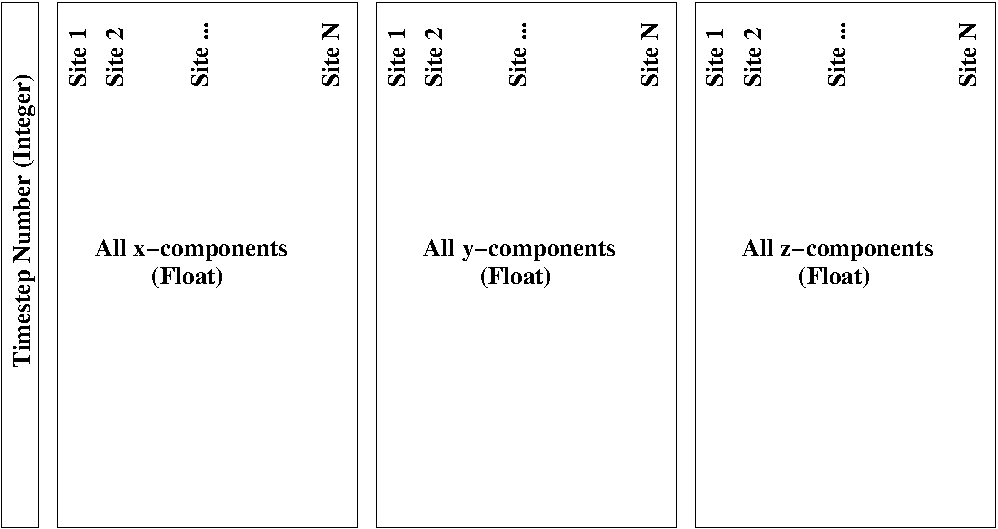
\includegraphics[width=10cm]{file_structure.pdf}
\end{center}
\caption{\label{fig:filestructure}The file structure for the dipole, and position files.}
\end{figure}

The anharmonicity file is only given in the SKIBIN format.
For each snapshot in the trajectory they contain first an integer typically containing the number of the snapshot. This integer is not used in the calculation, but can be used for control purposes.
Then the diagonal anharmonicities are then given in floats.

The overtone file is only given in the SKIBIN format.
For each snapshot in the trajectory they contain first an integer typically containing the number of the snapshot. This integer is not used in the calculation, but can be used for control purposes.
Then the overtone transition dipoles are then given in floats. Only the same site overtone transition dipoles are given. Transitions like $\langle 1\mid\mu\mid 12\rangle$ are determined by the harmonic rules.

The transition polarizability file which is not available in the SKIBIN format 
has the following format. For each snapshot in the trajectory they contain first an integer 
typically containing the number of the snapshot. This integer is not used in the calculation, 
but can be used for control purposes. Then the xx components of the transition polarizability
matrix are given in floats, followed by the yy and zz components. 

The position files are available in the GROBIN format and used to store either the center positions of the chromophores or the positions of the two sites in each chromophore defining the extended dipole coupling. This file is used when calculating CD spectra, excition diffusion, or when using the on-the-fly coupling calculations. The structure of the file is as for the dipole files (see Figure \ref{fig:filestructure}).

\noindent
\underline{GROASC:}\\
The energy file contain one Hamiltonian snapshot for each line. The upper tridiagonal matrix is saved and each number is separated by a space. The transition dipoles are stored in one file. Each line contains one snapshot with the numbers separated by a space. All the x components for one snapshot are stored first followed by the y and z components. Only the single excitation Hamiltonian and the transition dipoles from the ground state to the singly excited state are saved.

\noindent
\underline{MITASC:}\\
The energy file contain one Hamiltonian snapshot for each line. The whole square matrix is saved and each number is separated by a tab. The transition dipoles are stored in one file for each cartesian component. Each line contains one snapshot with the numbers separated by a tab. Only the single excitation Hamiltonian and the transition dipoles from the ground state to the singly excited state are saved.

\noindent
\underline{MITTXT:}\\
The energy file contain one row of the Hamiltonian snapshot for each line. The whole square matrix is saved and each number is separated by a space. Snapshots are separated by an empty line. The transition dipoles are stored in one file for each cartesian component. Each line contains the cartesian coordinates of one transition dipole. The numbers separated by a space. Snapshots are separated by an empty line. Only the single excitation Hamiltonian and the transition dipoles from the ground state to the singly excited state are saved.

\noindent
\underline{SPECTRON:}\\
In the energy file each snapshot is stored after a line containing the word SNAPSHOT and the number
of the snapshot (starting from 1). After this the upper tridiagonal matrix of the Hamiltonian snapshot is stored with one row on each line. The numbers are separated by a space. The dipole file also contain a line with the word SNAPSHOT and the number of that snapshot. This is followed by the transition dipoles stored with the x, y and z components for each site on one line separated by a space. Only the single excitation Hamiltonian and the transition dipoles from the ground state to the singly excited state are saved.


\subsection{NISE (Full nonadiabatic simulation)}
The nonadiabatic linear and third-order response can be simulated with the 'NISE' program utilizing the numerical integration of the Schr\"odinger equation (NISE) approach\cite{Jansen.2006.JPCB.110.22910,Jansen.2009.ACR.42.1405}. The sparse and double excited state propagation is described in \cite{Jansen.2010.JCP.132.224503}.
The coupling propagation scheme is described in \cite{Liang.2012.JCTC.8.1706}.
The program require the Hamiltonian trajectory in binary format.
The NISE program use the following input:\\
\begin{description}
\item [Hamiltonianfile] [File name]
\item [Dipolefile] [File name]
\item [Alphafile] [File name] (Only needed for SFG calculations)
\item [Anharmonicfile] [File name]
\item [Overtonedipolefile] [File name]
\item [HamiltonianType] [Full/Coupling/TransitionDipole/ExtendedDipole] (Full is the default)
\item [Couplingfile] [File name]
\item [PDBfile] [File name]
\item [Length] [Number of snapshots in trajectory] 
\item [Samplerate] [Number of snapshots between ensemble averaging]
\item [Lifetime] [The life time in fs]
\item [Timestep] [The length of each timestep in fs]
\item [RunTimes] [t1 max] [t2] [t3 max, all in timesteps]
%\item [MinTimes] [t1 min] [t2 min] [t3 min, all in timesteps, t1 min and t3 min should be 0]
%\item [MaxTimes] [t1 max] [t2 max] [t3 max, all in timesteps, t2 max should equal t2 min+1]
%\item [TimeIncrement] [dt1] [dt2] [dt3, all in timesteps, default 1]
\item [Threshold][The threshold for the sparse matrix approximation, typical value 0.001]
\item [Anharmonicity] [0 = anharmonicities from file used, all other values result in the use of a fixed anharmonicity with that value]
\item [Singles] [Number of singly excited states]
\item [Propagation] [Sparse/Coupling default is Sparse] (Coupling recommended for fast calculations)
\item [Couplingcut] [Value in cm$^{-1}$ below which the couplings are neglected, default 0, only used in the Coupling propagation scheme]
\item [Trotter] [The number of trotter steps in the Paarmann approximation for double excited 
states, 5 recommended for the Sparse propagation scheme, for the Coupling propagation scheme this is the general number of trotter steps the recommended value is then 1 ]
\item [MinFrequencies] [minw1] [minw2] [minw3, all in reciprocal cm]
\item [MaxFrequencies] [maxw1] [maxw2] [maxw3, all in reciprocal cm]
%\item [Static] [Minimum frequency] [Maximum frequency] [Bin size for 1D static spectrum]
\item [Technique] [Absorption / DOS / Luminescence / CD / 2DIR / GBIR / SEIR / EAIR / noEAIR / 2DUVvis / GBUVvis / SEUVvis / EAUVvis / noEAUVvis / Pop / Dif / Ani / Analyse, these techniques are explained in Section \ref{chap:techniques}]
\item [FFT] [Number of points on each axis in 2DFFT, if bigger than max times zero padding is used]
%\item [Timevariables] [1/2/3 First time to Fourier transform, should be 1] [1/2/3 Second time to Fourier transform, should be 3]
\item [Format] [Matlab/Dislin/Gnuplot For Matlab format rephasing and non-rephasing spectra are not added] 
\item [BeginPoint] [The number of the first sample calculated in this run]
\item [EndPoint] [The number of the last sample calculated in this run, if this keyword is left out all samples will be included]
\item [Project] (Should be followed by either two new lines specifying the sites to project on directly in the file or one line specifying the filename of a file to read the site numbers from. In the first case the first line should read Sites [Number] identifying how many sites are included in the projection and the second line with a list of integer numbers identifying the sites included counting from zero. In the other case the following line should read Projectfile [Name], where the file named [Name] contain the number of sites on the first line and then a list of the site numbers.)
\item [PrintLevel] [0 / 1 / 2 ] (Default is 0, the higher number the more detailed (timing) info is given.)
\end{description}

The minimum and maximum frequencies are used for two things. First, the average of minw1 and maxw1 are used to shift the frequencies during the simulation. By shifting all transitions by the
average the oscillations of the time-evolution are reduced and the simulations can be performed with
longer distance between the time points. Second, the output is reduced to frequencies within the
min and the max which reduce file size.

The lifetime is currently only applied during the coherence times ($t_1$ and $t_3$ ) according 
to the formula in \cite{Liang.2012.JCTC.8.1706}. The waiting time dependence can trivially be accounted for by 
multiplying the whole spectrum with $\exp( -t_2 /T_1 )$.

The HamiltonianType allow the use of different ways to store the Hamiltonian trajectories. The default setting is Full, where the full Hamiltonian is given in the Hamiltonianfile, if Coupling is specified the couplings are assumed to be constant and given in the Couplingfile. The Hamiltonianfile then contain the trajectory of fluctuating diagonal elements. If TransitionDipole is specified the couplings are calculated on the fly using the transition-dipole coupling scheme. The chromophore positions must then be provided in the Positionfile and the transition-dipoles in the Dipolefile. As for the Coupling method the HamiltonianFile then only contains the diagonal elements. The dipoles are then assumed in Debye and Positions in \AA ngstr\"{o}m. If ExtendedDipole is selected the extended-dipole coupling scheme is used to calculate coupling on the fly. The dipole magnitude is then taken from the Dipolefile. The position of the two transition point-charges must be provided in the Positionfile, with the first point corresponding to odd timepoints and the second point corresponding to even timepoints.

The double excitation Hamiltonian is propagated using the Trotter formula scheme\cite{Paarmann.2008.JCP.128.191103,Jansen.2010.JCP.132.224503}.

During the calculation the program will create a log file called NISE.log. For linear techniques this file will be updated every time a new sample has been calculated. The update contains timing information and
therefore allows for the estimation of when the complete calculation finishes. For 2D techniques the timing information will given directly in the output file tracking the progress percentage.

For exciton diffusion calculations an additional input file containing the site positions is needed.
This file should be named Position.bin and have the following format. The first entry should be the
size of the box in float (all sides are assumed equally long). This is followed by the x, y, and z coordinates for each site again in floats. After the coordinates of the first snapshot the coordinates
for the second follows directly and the coordinates for all snapshots should be stored.

%For SFG, 2DSFG, and linear dichroism calculations the principle axis is assumed to be the z-axis. The SFG calculations only support the calculation of $\chi^{(2)}_{zzz}$ and $\chi^{(2)}_{xxz}$, which require the diagonal elements of the transition polarizability tensor (given in the alpha file). For 2DSFG $\chi^{(4)}_{zzzzz}$ and $\chi^{(2)}_{zzzxx}$ are currently calculated.

\subsection{Program output}
The linear absorption calculation provides the linear response function in time domain in the file TD\_Absorption.dat 
and the linear dichroism response function in time domain in the file RLD.dat. The first 
column is the time in femto seconds. The other columns are the real and imaginary parts 
of the response function. It is recommended to check that these have decayed to a small 
value close to zero in the calculated time interval. If this is not the case the system has 
not lost its coherence within the time determined by t1 max and the spectrum will be 
too broad. The linear absorption is given in the file Absorption.dat and the linear dichroism in 
the file LDIR.dat. The first line is the frequency in wavenumbers, the second line is the 
absorption spectrum, and a third line contain zeroes. For the linear dichroism calculation 
the z-axis is assumed to be the unique axis. 

%The SFG calculation provides the second order response function in time domain in  the files RSFG\_zzz.dat and RSFG\_xxz\_yyz.dat. The first column is the time in femto seconds. The other columns are the real and imaginary parts of the response function.  It is recommended to check that these have decayed to a small value close to zero in the calculated time interval. If this is not the case the system has not lost its coherence within the time determined by t1 max and the spectrum will be too broad. The frequency domain response functions are given in the files SFG\_zzz.dat and SFG\_xxz\_yyz.dat. The first line  is the frequency in wavenumbers, the second line is the absorption spectrum, and a third line contain zeroes. The z-axis is assumed to be the unique axis.

The 2D calculations (2DIR and 2DUVvis) provides the files R(par/per/cro)(I/II).dat. These files contain the time domain
third-order response functions for different polarization directions \cite{Hochstrasser.2001.CP.266.273,Zanni.2001.PNAS.98.11265}.
The first three columns are the times t1, t2, and t2 in femtoseconds.
The two last columns are the real and imaginary parts of the response functions. The frequency domain
response functions are found using a double Fourier transform (see section \ref{sec:Fourier}).
It is recommended to check that the response function has decayed within the calculated time intervals.

%The 2DSFG calculation stores the $\chi^{(4)}_{zzzzz}$ signal in Rpar(I/II).dat, while the $\chi^{(4)}_{zzzyy}$ signal is stored in Rper(I/II).dat. The files are essentially identical to the normal 2D response files and are Fourier transformed in the same way (see section \ref{sec:Fourier}).

The population transfer calculation provides two files. Pop.dat contain two columns. The first is the
time in femtoseconds the second is the probability that if a site was initially excited it is still excited
after the given time. This is averaged over all sites. The file PopF.dat contain more detailed information.
The first column is the time. The following columns are the probability that if a particular site was excited
initially other sites are excited later. The first N columns are the populations of the N sites following an initial excitation of the first site. Then follows the populations after excitation of the second site etc. This file might be a very large file for big systems.

For the exciton diffusion the output file is Dif.dat It has three columns. The first is the time in femto seconds. The second column is the mean square displacement of the wave function assuming that
one site is initially excited. The third column is the mean square displacement of the center of the 
wave function assuming that one site is initially excited. The program averages over all sites as
initial sites. One should be aware that periodic boundary conditions are applied in this calculation
and the mean square displacements will saturate \cite{Jansen.2010.JCP.132.224503}.

For the integrated anisotropy calculation the output file is Ani.dat. It has three columns. The first is the time in femtoseconds. The second is the integrated anisotropy and the last is the orientational correlation function.

The Hamiltonian analysis provides the delocalization length/size according to the def- 
inition of Thouless \cite{Thouless.1974.PR.13.93} directly in the program standard output. 

\section{Fourier transform \label{sec:Fourier}}
The 2DFFT program use the same input as the NISE program.
Fourier transformed response is written in files named Rw(par/per/cro).(I/II).dat, where par, per, and cro denote parallel, perpendicular and cross polarized signals. I and II denote the $k_I$ and $k_{II}$ contributions. When Dislin format is used the 2D correlation spectrum is saved in the files 2D.(par/per/cro).dat and the 'broad pump narrow probe' pump probe signal is stored in PP.(par/per/cro).dat.
The first column is $\omega_1$, the second is $\omega_2$, the third is the dispersive signal, and the
last column is the absorptive signal. Perl scripts connected with Dislin are available for plotting or the
user can use his or her favorite plotting program. The Dislin format is also used by the python plotting code included in the tutorial files.
The Gunplot output is only differing from the Dislin format in an empty line following ach new value of $\omega_1$. A Gnuplot example file is included in the tutorial. A python plotting script which use the Dislin output format file is included. The cover picture 
of the manual is generated with this python script.
 For Matlab format only the Rw files are created. These
then contain a matrix with the response. An additional file waxis.dat is created with the values of the
frequencies.




\chapter{Tutorial}
A tutorial example exists for two coupled chromophores. To activate this you need to run {\tt make example}s in the {\tt build} directory. The tutorial files are located in the folder {\tt examples/tutorial}. The program stochastic creates the input 
trajectories in GROASC format and input files can be found for converting to GROBIN and for the
calculation of linear and two-dimensional spectra. The stochastic code allow the user to construct
a simple trajectory for two coupled three level system. It is assumed that these levels are coupled
to a set of overdamped Brownian oscillators \cite{Mukamel.1995.B01}.
The user can vary the length of the trajectory, the duration of the time interval between snapshots, the 
width of the frequency distribution, the correlation time, and the degree of correlation between the
two three level system fundamental frequency fluctuations. The energy difference and the average frequency for the two fundamental frequencies can be adjusted as can the coupling between them.
The angle between the assumed fixed transition dipoles can be adjusted as well. An example for
parameters is given in the script named run. 

After generating the frequency trajectory with the stochastic program one can look at the generated
trajectories in Energy.tex and Dipole.tex. The should the be converted to binary input for the NISE
program. This is done with the translate program with the input given in the file inpTra.
The command line entry:
\begin{verbatim}
~/NISE_2017/bin/translate inpTra
\end{verbatim}
will accomplish this. (It is assumed that you installed NISE in your home directory. If the programme was installed somewhere else you need to run the programme from the alternative bin directory where it was installed.)

When the binary trajectory exist we can calculate the linear absorption using the input from the file input1D.
\begin{verbatim}
~/NISE_2017/bin/NISE input1D
\end{verbatim}
One should plot the output in TD\_Absorption.dat and Absorption.dat to get familiar with this. It is 
important that the response function has decayed almost completely within the simulated 
time to avoid ringing and other artifact in the spectrum. The program should finish in a 
about 10 seconds. The python script plot.py will plot both the response function and the absorption spectrum. Simply type {\tt python plot.py} assuming that python 3 is installed. Alternatively, you can plot the two first columns of each file with your own favourite plotting programme.

The linear dichroism signal can be calculated by changing the {\tt Technique} to {\tt LD} which generate corresponding files with the names TD\_LD.dat and LD.dat. In the turotial this is 
not so interesting as it is simply minus half of the absorption signal, since the dipoles are in the 
x, y plane and the unique angle for linear dichroism is defined to be the z-axis.

The two-dimensional infrared spectra are calculated with the input file input2D. This corresponds to the spectrum of two coupled three-level systems in this case, where the anharmonicity is 20 cm$^{-1}$ for both three-level systems as specified in the input2D file. The programme is executed with the command:
\begin{verbatim}
~/NISE_2017/bin/NISE input2D
\end{verbatim}
The percentage wise progress of the calculation can be followed in the output. One should expect that the calculation of one sample point takes about 10 seconds with the given settings. For a test about 100 samples are sufficient, while for nice spectra at least 1000 samples are needed. Typically more samples are needed for two-dimensional spectra than for linear absorption spectra and the more different distinct chromophore environments are present the more samples are needed. The given example should take about 15 minutes to simulate (of course depending on the computer).
If you have multiple cores on your computer you can run the MPI parallel version typing:
\begin{verbatim}
mpirun -n 4 ~/NISE_2017/bin/NISE input2D
\end{verbatim}
The number 4 tells mpi that the job should be split in 4. For this small system mpi is likely more efficient then OpenMP on typical computer architectures. The output of the NISE programme is the time domain response functions. To get the frequency domain spectra the 2DFFT program must be executed as described below.

The NISE code was originally build to consider coupled three-level systems, which is what is needed to simulate infrared spectra. If one want to simulate two-dimensional electronic spectra coupled two-level systems usually need to be considered. This can now be achieved with the 2DUVvis technique. Previously this was achieved by using an anharmonicity that moves the third-level out of the spectral window and sufficiently far away that the coupling between the third-level for each monomer and double excitations involving pairs of sites can be neglected \cite{Olbrich.2011.JPCB.115.8609,Liang.2012.JCTC.8.1706}. 

The 2D simulations can be performed in parallel using openMP. The program does this by distributing the calculations for different values of t1 on different CPUs. When running parallel it is advantageous to ensure that ([t1 max]+1) divided by the number of used CPUs is an integer number or slightly smaller than an integer number. To run the code parallel the OMP\_NUM\_THREADS variable has to be set equal to the number of CPUs that one want to use in the submission script (or if not running under a queueing system the variable has to be set in the used linux shell). On most clusters one should further specify to the queuing system how many CPUs are needed when submitting the job. The user is referred to the manual of the cluster used for this kind of information as it varies from system to system. For parts of the code, where the mkl library is used for solving eigen value problems these may be run in parallel as well by setting the MKL\_NUM\_THREADS variable equal to the number of CPUs used for this task. The general experience is that for small problems running parallel is not efficient. The mkl library also does not perform well on large numbers of CPUs, however, the 2D simulations were found to scale well up to about 32 CPUs in recent simulations on 864 coupled OH-stretch oscillators \cite{Shi.2016.PCCP}. For large problems the calculation of polarization contributions and samples can efficiently be spread over different CPUs and/or nodes for efficent massively parallel calculations.

The response functions calculated in time domain can be converted to frequency domain spectra using the double Fourier transform code with the same input as for the calculation of the response function.
\begin{verbatim}
~/NISE_2017/bin/2DFFT input2D
\end{verbatim}
The output can be visualized with one of the plotting scripts provided with the tutorial. The recommended metod is using the {\tt plot2D.py} python script, which is written to plot the parallel polarization spectra. The line {\tt Data = np.loadtxt('2D.par.dat')} in the beginning of the script can be changed to load and plot one of the other data files (perpendicular spectrum {\tt 2D.per.dat} or cross polarization {\tt 2D.cro.dat'}. The plot at the cover of the manual is the parallel polarization 2DIR spectrum obtained from the tutorial.

The user is encouraged to play with the settings of the run script in the tutorial to get familiar with the code.
The simple example can also be useful for getting familiar with the basics of two-dimensional spectroscopy in particular regarding the effects of coupling, correlation, relative angles between
coupled chromophores.

The delocalization length \cite{Thouless.1974.PR.13.93} can be calculated with the analysis option as given in 
the example input file inputAnalyse. Note that for including the complete trajectory [t1 
max] should be 1. 
\begin{verbatim}
~/NISE_2017/bin/NISE inputAnalyse 
\end{verbatim}
%A separate tutorial exists for the SFG part of the code. The script for creating the  trajectory is called runSFG. The input files for the translate and NISE3 programs are  called inpTraSFG, and input(2D)SFG, respectively. In this tutorial two sites are given. The  transition dipole of the first is parallel to the z-axis and pointing in the positive direction. The angle with the other dipole can be specified in the script. The transition polarizability components for both sites are $\alpha_{xx}$ = $\alpha_{yy}$ = 1 and $\alpha_{zz}$ = 10. The frequency fluctuation parameters can be specified as in the main tutorial.

A more extensive set of tutorials can be found at https://github.com/GHlacour/NISE\_Tutorials. This include examples for the LH2 light-harvesting system.
This tutorial repository also contains useful scripts for plotting the spectra calculated with this code.


\chapter{\label{chap:techniques}Details on the available techniques}
In this Chapter, more details on special options and the theory behind each technique is given. The techniques marked with a star (*) are implemented with OpenMP and MPI options (see \cite{Sardjan_2020}), while techniques implemented with OpenMP options are marked with a plus (+). All other techniques are implemented as single CPU. 
\section{Analyse}
The Hamiltonian is analysed and different statistical properties are provided including the average delocalization size of Thouless \cite{Thouless.1974.PR.13.93}. This inverse participation ratio (IPR) is expressed as:
\begin{equation}
	D_{IPR}=\left\langle\frac{1}{N}\sum_i\left(\sum_j |c_{ij}|^{4}\right)^{-1}\right \rangle.
\end{equation}
In a file named Analyse.dat statistics is given for each site including. This include the average energy and the standard deviation. The average coupling strength (signed sum of all couplings of a given site with all other sites) and the standard deviation of this quantity.
In a file named Av\_Hamiltonian.txt. The average Hamiltonian is stored as a single snapshot in the GROASC format.
Furthermore, the density matrix is calculated for the spectral region defined by the upper and lower bounds of \textbf{MinFrequencies} and \textbf{MaxFrequencies}. This is done both with and without a weight determined by the contribution to the absorption spectrum as:
\begin{equation}
\rho_{ij}=\sum_k \Big\langle c_{ik}^* c_{jk}  \Theta(\omega_{k}-\omega_{min})\Theta(\omega_{max}-\omega_k)\Big\rangle
\end{equation}
Where $c_{jk}$ is the wavefunction coefficient of eigenstate $k$ on site $j$ and $\omega_k$ is the wavenumber associated with that eigenstate. The brackets symbolize the ensemble average over the trajectory.
\begin{equation}
\rho^{\textrm{spectral}}_{ij}=\sum_k \Big\langle |\vec{\mu}_k|^2 c_{ik}^* c_{jk}  \Theta(\omega_{k}-\omega_{min})\Theta(\omega_{max}-\omega_k)\Big\rangle
\end{equation}
Here $\vec{\mu}_k$ is the transition-dipole vector of eigenstate $k$. This weighted density matrix, thus, emphasizes the states contributing to the absorption spectrum in the given spectral window. These density matrices are stored in the files named LocalDensityMatrix.dat, and SpectralDensityMatrix.dat. The former should be identical to the unit matrix if the full region of all eigenstates is included.

\section{Pop (population transfer)}
The population transfer is calculated between sites. In general, this is governed by the equation:
\begin{equation}
P_{fi}(t)=\langle |U_{fi}(t,0)|^2 \rangle
\end{equation}
Here $f$ and $i$ are the final and initial sites. Generally two files are generated. In Pop.dat average of the population remaining on the initial site ($P_{ii}$) is calculated resulting in a value starting at 1 (all popiulation is on the initial state) and decaying to the equilibrium value 1/N (equal population on all states). In the PopF.dat file a full matrix op all combinations of initial and final states is given. The columns start start with the first initial state and all possible final states continuing to the second possible initial state and all possible final states. This file may be very large for large system sizes!
\section{Dif (diffusion)$^{+}$}
The mean square displacement of excitons are calculated using the positions provided in the Positions file. Periodic boundary conditions are applied assuming a cube box. The box size must be provided in the first column of the Positions file.
Two diffusion properties are calculated. The diffusion of the exciton center is calculated by calculating the center of the excitation given it started on a specific site $j$: $x_{\textrm{ex},i}(t)=\langle \sum_j (x_j(t)-x_i(0)) |U_{ji}(t,0)|^2$ and then determining the mean square displacement as $MSD_{\textrm{ex}}(t)=\langle \sum_i  x_{\textrm{ex},i}(t)^2\rangle$. The other measure is based on the probability of starting on one site and being detected on another site $MSD_{\textrm{site}}(t)=\langle \sum_{ji} (x_j(t)-x_i(0))|U_{ji}(t,0)|^2\rangle$. $MSD_{\textrm{site}}(t)$ is stored in the second column of the Dif.dat output file and $MSD_{\textrm{ex}}(t)$ is stored in the third column. The first column contain the time in femtoseconds. The unit for the mean square displacements is the distance unit provided on the position file (\AA ngstr\"{o}m recommended) squared per femtosecond. 
\section{Ani (anisotropy)}
Not implemented yet (check NISE\_2015)
\section{DOS$^{+}$}
The density of states is calculated using the response function:
\begin{equation}
	I(t)=\langle\textrm{Tr}U(t,0)\rangle\exp(-t/T_1).
\end{equation}
Both the real and imaginary parts are stored. The Fourier transform is the frequency domain density of states, which is stored in the file DOS.dat. $T_1$ is the lifetime, which is often simply used as an appodization function to smoothen the spectrum.
\section{Absorption}
The linear absorption is calculated using the first-order response function \cite{Duan_2015}
\begin{equation}
	I(t)=\sum_{\alpha}^{x,y,z}\langle\mu_{\alpha}(t)U(t,0)\mu_{\alpha}(0)\rangle\exp(-t/T_1).
\end{equation}
Both the real and imaginary parts are stored. The Fourier transform is the frequency domain absorption, which is stored in the file Absorption.dat. $T_1$ is the lifetime, which is often simply used as an appodization function to smoothen the spectrum. 
\section{Luminescence}
The luminescence is calculated using the first-order response function
\begin{equation}
	I(t)=\sum_{\alpha}^{x,y,z}\langle\frac{1}{Z}\mu_{\alpha}(t)U(t,0)\exp(-H(0)/k_BT)\mu_{\alpha}(0)\rangle\exp(-t/T_1).
\end{equation}
Both the real and imaginary parts are stored. The Fourier transform is the frequency domain luminescence, which is stored in the file Luminescence.dat. $T_1$ is the lifetime, which is often simply used as an appodization function to smoothen the spectrum. The Boltzmann term containg the Hamiltonian at time zero ($H$) and the temperature (to be specified in the input) ensure the emission from a termalized population of the excited state ignoring a potential Stoke's shift and effects of vibronic states. The spectrum is normalized with the partition function ($Z$). 
\section{LD (linear dichroism)}
The linear dichroism is calculated identically to the linear absorption except the average of the absorption in the x and y directions is subtracted from the absorption in the z direction. This corresponds to a perfect linear dichroism setup, where the molecules are aligned along the z-axis.
\section{CD (circular dichroism)$^{+}$}
The circular dichroism is calculated using the first-order response function
\begin{equation}
	I(t)=\sum_{\alpha}^{x,y,z}\sum_{nm}\langle r_{nm}\mu_{\alpha,n}(t)\times[U(t,0)\mu_{\alpha,m}(0)]\rangle\exp(-t/T_1).
\end{equation}
Both the real and imaginary parts are stored. The Fourier transform is the frequency domain absorption, which is stored in the file Absorption.dat. $T_1$ is the lifetime, which is often simply used as an appodization function to smoothen the spectrum. Note that the positions of the chromophores must be provided in the Positions file. The calculation does \textit{not} account for periodic boundary positions and the positions must at all times along the position trajectory be specified accordingly.
\section{Raman}
The Raman response is calculated as \cite{Torii.2002.J.Phys.Chem.A.106.3281,Shi.2012.J.Phys.Chem.B.116.13821}
\begin{equation}
        I^{VV/VH}(t)=\sum_{a,b,c,d}^{x,y,z}A^{VV/VH}_{abcd}\langle\alpha_{ab}(t)U(t,0)\alpha_{cd}(0)\rangle\exp(-t/T_1),
\end{equation}
where $A^{VV/VH}_{abcd}$ is the orientational weighting factor as defined in Ref. \citenum{Shi.2012.J.Phys.Chem.B.116.13821}. 
Both the all parallel (VV) and perpendicular (VH) components are calculated. The calculation require that the transition-polarizability file is provided with all six independent components stored. The data are stored in the files Raman\_VV.dat and Raman\_VH.dat.
\section{SFG (sum-frequency generation)}
Not implemented yet (check NISE\_2015)
\section{2DIR$^{*}$ (two-dimensional infrared)}
This calculates the two-dimensional infrared spectra assuming coupled three level systems. The techniques GBIR (ground state bleach), SEIR (stimulated emission), and EAIR (excited state absorption) provides these contributions separetely. Furthermore the sum of the ground state bleach and the stimulated emission can be calculated with the noEA technique keyword. The expressions for the response functions are given in ref. \cite{Jansen.2006.JPCB.110.22910}.
\section{2DSFG (two-dimensional sum-frequency\\ generation)}
 Not implemented yet (check NISE\_2015)
\section{2DUVvis$^{*}$ (two-dimensional electronic\\ spectroscopy)}
This calculates the two-dimensional infrared spectra assuming coupled two level systems. The techniques GBUVvis (ground state bleach), SEUVvis (stimulated emission), and EAUVvis (excited state absorption) provides these contributions separetely. Furthermore the sum of the ground state bleach and the stimulated emission can be calculated with the noEAUVvis technique keyword. 
\section{2DIRRaman$^{*}$}
This calculates the two-dimensional infrared raman spectra assuming coupled three level systems. The techniques 2DIRraman1 (rephasing), 2DIRraman2 (non-rephasing 1), 2DIRraman3 (non-repasing 2) provides these contributions separetely. The rephasing diagram and the non-rephasing diagrams are stored separately as they cannot be directly added. % The expressions for the response functions are given in ref. \cite{}.
\section{2DFD (fluorescence detected two-dimensional\\ spectroscopy)}
 The 2DFD spectrum can be calculated in the approximation that all exciton pairs annihilate to produce a single exciton long before fluorescence occur with the noEAUVvis technique. The response functions governing this technique are provided in ref. \cite{Kunsel_2018}.


\chapter{Information for developers\label{chap:developers}}
Contributions from developers are welcome. The code is available on
github:\\ (https://github.com/GHlacour/NISE\_2017). It is advisable to contact the main developer before planning contributions to avoid competing contributions. All new techniques should be added in new separate files which are called from the main {\tt NISE.c} code. 
Implementations should as far as possible make use of existing modules for reading input and data. New propagation schemes should be added in {\tt propagate.c}, Hamiltonains should be added through {\tt read\_trajectory.c} generally useful additions should made in the {\tt NISE\_subs.c} module. Projection schemes should be added in {\tt project.c}.

Bugs, feature requests, and other issues can be reported through the Issues option on GitHub or by contacting the main developer directly.


\chapter{Acknowledgement}
The following people are kindly acknowledged for their contribution through helpful discussions, ideas, and feedback:
Foppe de Haan, Arend Dijkstra, Alexander Paarmann, Carsten Olbrich, Jim Skinner and his group, Lu Wang, Carlos Baiz, Chungwen Liang, Santanu Roy, Ana V. Cunha, Andy Sardjan, and Ariba Javad. 

The NWO is gratefully acknowledged for financial support making is possible to write the initial versions of this code through VENI and VIDI grants. 
 
\bibliography{Merged2016}

\end{document} 
